\chapter[Session 2: Thread]{Threads}\label{chap:session2}
\chaptermark{Threads}
The second session of this lab will contain some exercises about threads. In session \ref{chap:session1} you learned about process and how they work. In this assignment you will use threads and these threads will be used in all other session of this lab. The objectives of this session are listed below.
	\begin{itemize}
		\item Learn what a thread is and how you could create one
		\item Learn how you could use the I/O interface of the Raspberry Pi
	\end{itemize}

\section{Assignments}
In the previous assignment you already learned something about processes on a Linux system. In this second assignment you will learn something about threads. 

A thread is a basic unit of CPU utilisation; it comprises a thread ID, a program counter, a register set, and a stack. It shares with other threads belonging to the same process its code section, data section, and other operating-system resources, such as open files and signals. A traditional (or heavyweight) process has a single thread of control. If a process has multiple threads of control, it can perform more than one task at a time. Since each unique thread has its own memory, it is a lot faster to create and destroy threads. 

\begin{figure}
  \centering
  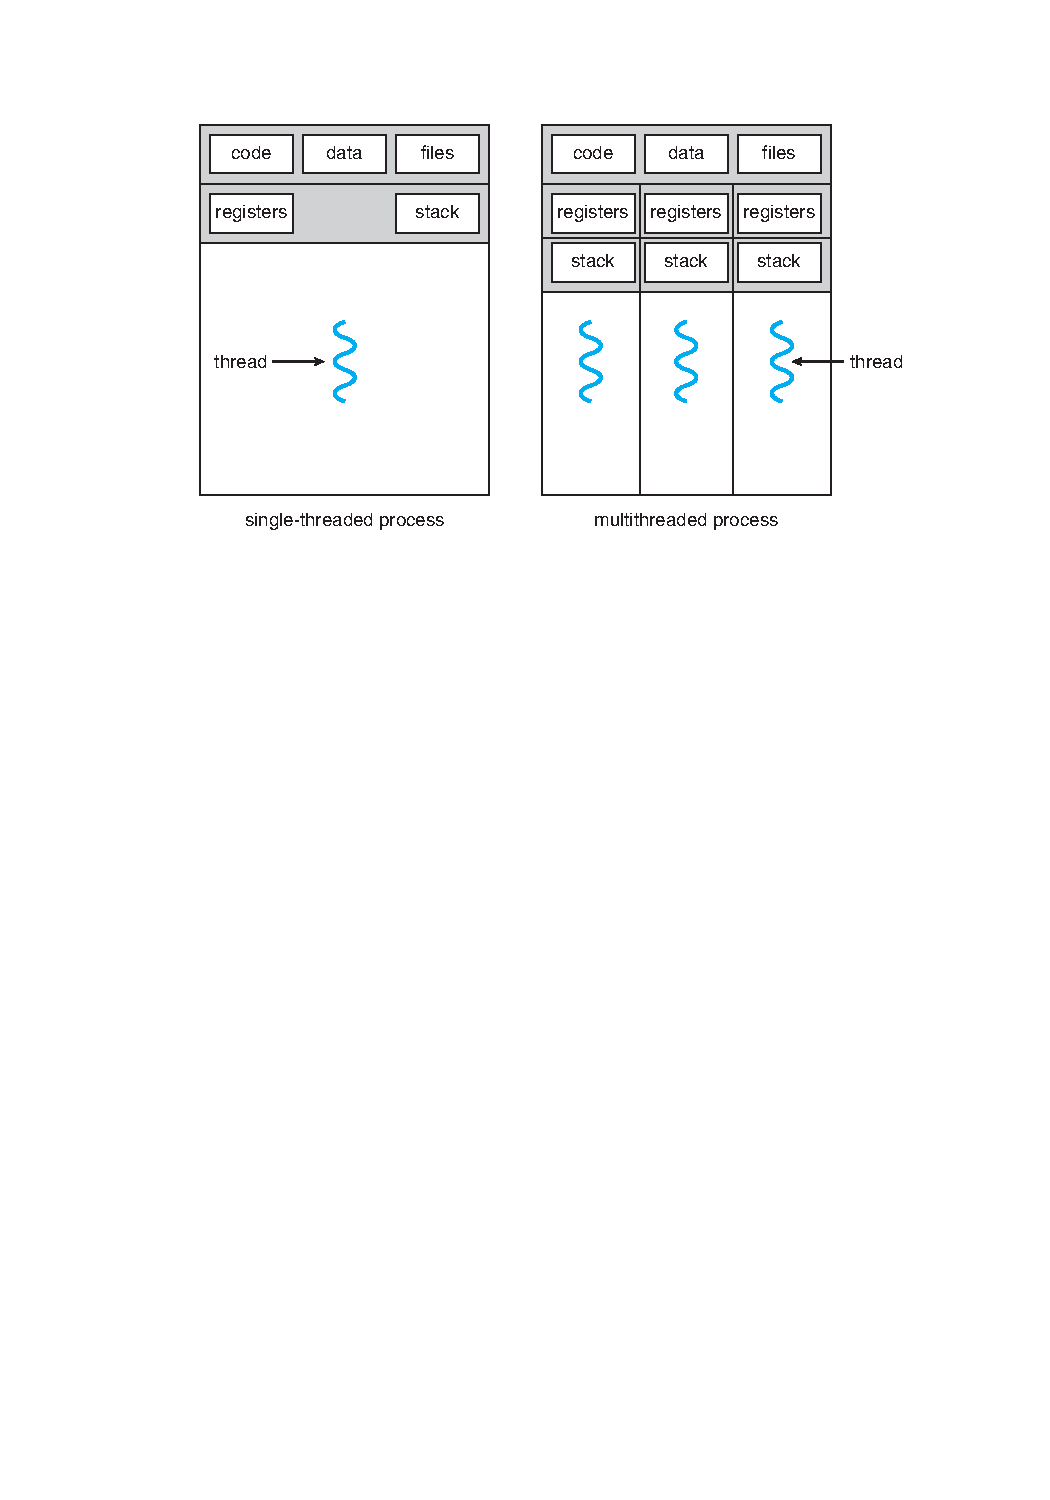
\includegraphics[width=.8\textwidth]{images/thread.pdf}
\caption{Single-Threaded and Multi-Threaded Processes}
\label{fig:thread}
\end{figure}

In this session you will learn how to create threads. The concept of threads will be further utilised by all the other assignments of this lab. The next session is about multithreading and the advantage of threads above processes.

\subsection*{Using I/O on Raspberry Pi}\label{sec:io-intro}
This tutorial will state information with regards to the input/output (I/O) functionalities of the Raspberry Pi. To make it easy, we will use a library which provides a set of functions to communicate with the I/O pins of the Raspberry Pi. This lab will use the Wiring Pi library. This tutorial will mention the basic functions you have to use during this lab. If you want to use more advanced functions you could find a detailed reference on the website of WiringPi \url{http://www.wiringpi.com/reference}

Before using the WiringPi I/O library, you need to include its header file in your programs:

\begin{lstlisting}
#include <wiringPi.h>
\end{lstlisting}
Due to the fact that you will be using a non-standard library, do not forget to link the library when compiling your file. Therefore you could use the following line:

	\begin{codeblock}
		-I/usr/local/include -L/usr/local/lib -lwiringPi
	\end{codeblock}
When you have successfully included the library you are able use the WiringPi functions. The first thing you have to do is to call the function \code{wiringPiSetup()}:

\begin{lstlisting}
// Setup WiringPi
wiringPiSetup();
\end{lstlisting}
Once you have called the function \code{wiringPiSetup()} you are able to set the mode of the pins. Each pin can be set to several modes and therefor you have to select the right one in order to operate the pin correctly. To select the different pin modes you could use the function \code{pinMode(int pin, int mode);}:

\begin{lstlisting}
// Set LED1 pin to output
pinMode(LED1, OUTPUT);
\end{lstlisting}

Another function you will be going to use is the function to change the output value of the LED pins in order to turn the LED on or off. You could change the output value low or high by the function \code{digitalWrite (int pin, int value);}

\begin{lstlisting}
// Turn LED on
digitalWrite(LED1, HIGH);

// Turn LED off
digitalWrite(LED1, LOW);
\end{lstlisting}

The previously stated functions will allow you to turn the LED's on or off, more specifically the first function turns LED1 on, and the second one turns it off. The functions mentioned below can be used to control the LED's with a Pulse Width Modulated signal (PWM). PWM can be used to control the brightness of the LED's. Additionally PWM can be used to fade-in and fade-out the LED's. The LED's which you will be going to control with PWM signals must be initialised different than just turning LED's on and off. The function \code{softPwmCreate (int pin, int initialValue, int pwmRange);} is used to initialise the LED. In this function you have to enter a initial value (0 for off and 100 for fully  on) and the pwmRange which should be 100. 

The function \code{softPwmWrite(int pin, int value);} is used to update the PWM value of the LED. We use for PWM the soft PWM library because there is only one pin on the Raspberry Pi which allows hardware PWM. Soft PWM means a thread is created which controls the LED to the corresponding PWM value. Before you can use the functions for PWM you have to include the soft PWM library. \code{\#include <softPwm.h>}

\begin{lstlisting}
// Include headers
#include <wiringPi.h>
#include <softPwm.h>

// Initialise pin for PWM output
softPwmCreate(LED1, 0, 100);

// Update the PWM value of a LED
softPwmWrite(LED1, 50);
\end{lstlisting}

\subsection*{Assignment 2.1}
The objective of this assignment is creating a new thread. You have to include the POSIX Thread library in order to create a thread in your main function. The only thing you have to implement in your main function is the creation of a thread, waiting for the thread to finish and killing the program. The complete list of objectives of this assignment are listed below.
	\begin{objectives}
		Objectives for a correct implementation of Assignment 2.1
		
		The main function must create a thread, wait till the thread is finished and finally close the program. The objectives of the thread are listed below.
		\begin{itemize}
			\item Print the thread ID and function name of the thread
			\item Create a counter which counts from 1 to 10 and wait 1 second between each increment
		\end{itemize}
	\end{objectives}
	\signature

\subsection*{Assignment 2.2}
In this assignment you will - just as in assignment 2.1 - create a thread. Basically the same main functions can be used. However, instead of using a timer you will use the input/output port of the Raspberry Pi. In this assignment you have to use the output function of this port to blink multiple LED's. The objectives of this assignment are listed in the grey box below.
	\begin{objectives}
		Objectives for a correct implementation of Assignment 2.2
		
		The main function must create a thread, wait till the thread is finished and finally close the program. The objectives of the thread are listed below.
		\begin{itemize}
			\item Initialise the LED pins as output
			\item Create a certain pattern with the LED's
			\item Close the thread after 20 seconds
		\end{itemize}
		
		The pattern named above may be every pattern you want. It could be some difficult pattern or just simple blinking of LED's
	\end{objectives}
	\signature
	
\section{Bonus Question: Sudoku Solution Validator}
\label{sec:sudoku}
A Sudoku puzzle uses a 9 × 9 grid in which each column and row, as well as each of the nine 3 × 3 subgrids, must contain all of the digits 1···9. Figure \ref{fig:sudoku} presents an example of a valid Sudoku puzzle. This project consists of designing a multithreaded application that determines whether the solution to a Sudoku puzzle is valid.
There are several different ways of multithreading this application. One suggested strategy is to create threads that check the following criteria:
\begin{itemize}
\item A thread to check that each column contains the digits 1 through 9
\item A thread to check that each row contains the digits 1 through 9
\item Nine threads to check that each of the 3 × 3 subgrids contains the digits 1 through 9
\end{itemize}

\begin{figure}[hbp]
\centering
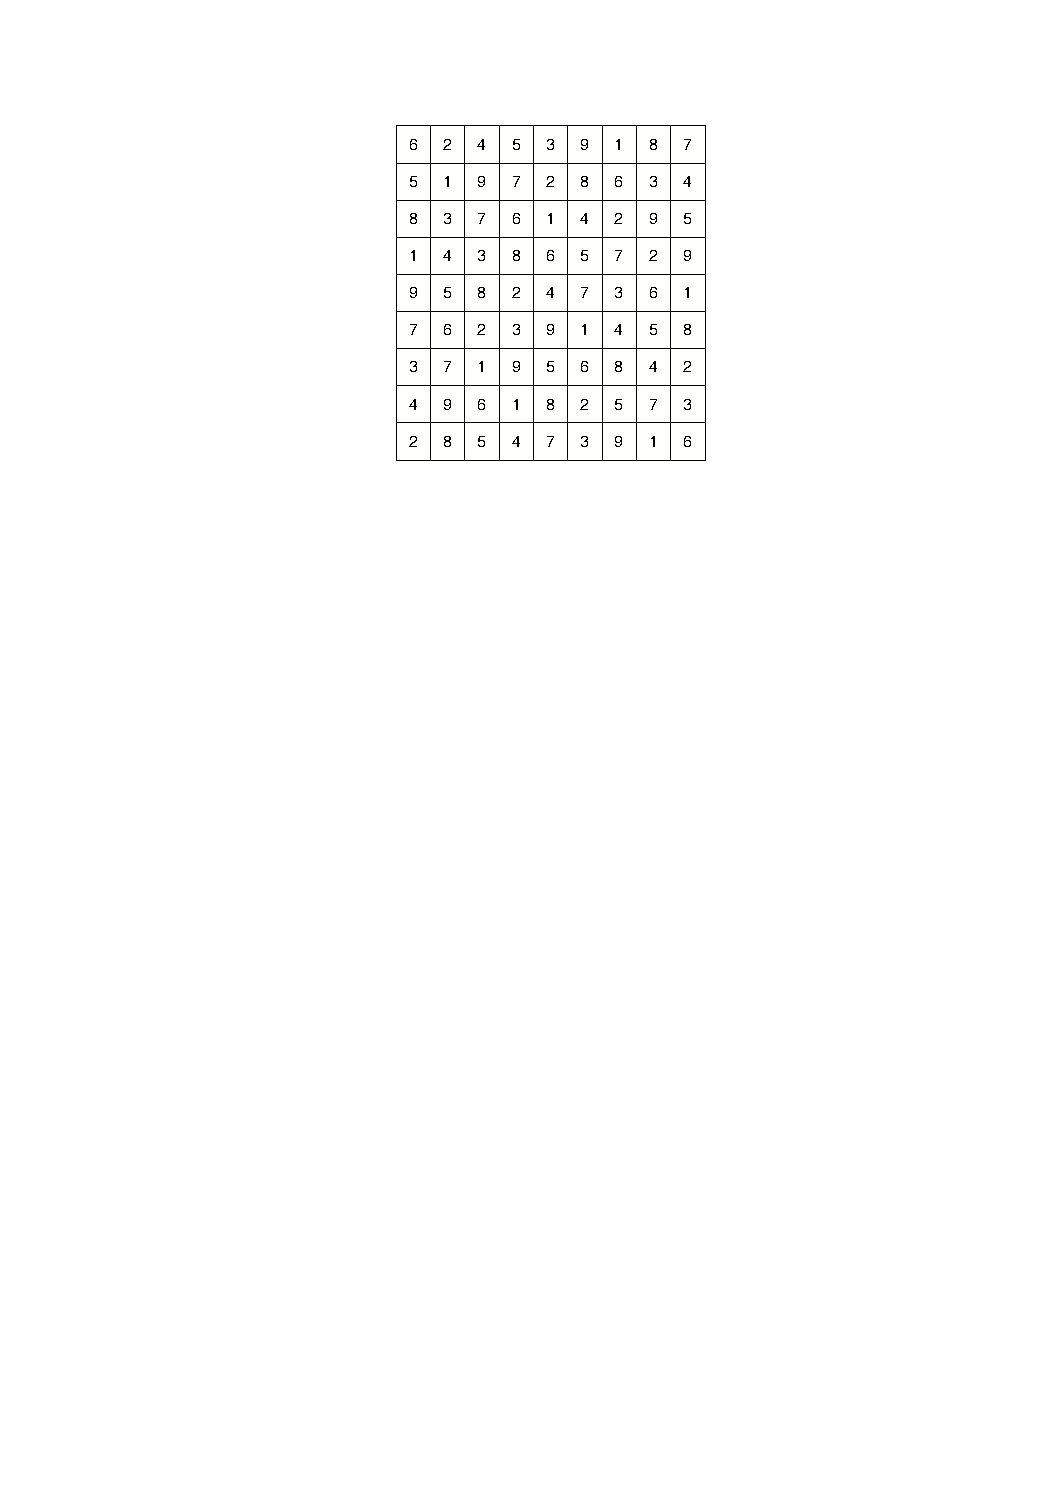
\includegraphics[width=0.5\textwidth]{images/sudoku.pdf}
\caption{Solution to a 9 x 9 Sudoku puzzle}
\label{fig:sudoku}
\end{figure}

This would result in a total of eleven separate threads for validating a Sudoku puzzle. However, you are welcome to create even more threads for this project. For example, rather than creating one thread that checks all nine columns, you could create nine separate threads and have each of them check one column.

\subsection*{Passing Parameters to Each Thread}
The parent thread will create the worker threads, passing each worker the location that it must check in the Sudoku grid. This step will require passing several parameters to each thread. The easiest approach is to create a data structure using a struct. For example, a structure to pass the row and column where a thread must begin validating would appear as follows:
\begin{lstlisting}
/* structure for passing data to threads */ 
typedef struct {
   int row;
   int column; 
} parameters;
\end{lstlisting}

Both Pthreads and Windows programs will create worker threads using a strategy similar to that shown below:
\begin{lstlisting}
parameters *data = (parameters *) malloc(sizeof(parameters)); 
data->row = 1;
data->column = 1;
/* Now create the thread passing it data as a parameter */
\end{lstlisting}

The data pointer will be passed to the \code{pthread create()} (Pthreads) function, which in turn will pass it as a parameter to the function that is to run as a separate thread.

\subsection*{Returning Results to the Parent Thread}
Each worker thread is assigned the task of determining the validity of a particular region of the Sudoku puzzle. Once a worker has performed this check, it must pass its results back to the parent. One good way to handle this is to create an array of integer values that is visible to each thread. The ith index in this array corresponds to the ith worker thread. If a worker sets its corresponding value to 1, it is indicating that its region of the Sudoku puzzle is valid. A value of 0 would indicate otherwise. When all worker threads have completed, the parent thread checks each entry in the result array to determine if the Sudoku puzzle is valid.\\
\signature

